% =====================================================================
%  2026-05-06 — 環境建置 + 麵包板 TIA + PySpice 模擬交叉驗證
% =====================================================================

\subsection*{今日目標}

\begin{itemize}[leftmargin=2em,itemsep=0pt]
  \item 把 4/19 構想中的 \textbf{BPW34 + MCP6004 TIA} 真的接在麵包板上。
  \item 同時建好 \textbf{PySpice + ngspice} 的模擬環境,把同一個電路在 SPICE 裡跑一次,
        看實際量測能不能對得上 \(V_\text{OUT} = I_\text{photo} R_F\)。
  \item 用 AC sweep + transient 兩種模擬,挑出能同時保住 ProMotion 120 Hz
        與 OLED PWM \(\SI{20}{\kilo\hertz}\) 的補償電容 \(C_F\)。
\end{itemize}

\subsection*{Python 模擬環境建置}

底層用 \texttt{uv} 管的 Python 專案,核心依賴 \texttt{pyspice}\,\(\geq\,\)1.5、
\texttt{numpy}、\texttt{matplotlib}、\texttt{schemdraw};系統面要裝 Debian 的
\texttt{libngspice0} 與 \texttt{ngspice}(\texttt{spinit} 與 \texttt{*.cm} codemodel 必備,
否則 Microchip macromodel 內的 PSpice \texttt{POLY} E/G-source 無法被翻成 XSPICE A-block)。

今天和 Claude Code 一起對接時,踩了三個 ngspice 與 PySpice 接合面的坑,
每個都得 patch 才能順利跑模擬,記下來以便日後查找:

\begin{enumerate}[leftmargin=2em,itemsep=2pt]
  \item \textbf{libngspice SONAME 問題}。 PySpice 1.5 的 cffi loader 寫死了
        \texttt{dlopen("libngspice.so")},但 Debian 的 \texttt{libngspice0}
        只提供 SONAME 版本 \texttt{libngspice.so.0}(無版本符號連結屬於 \texttt{-dev} 套件)。
        \emph{Fix:} 在 \texttt{import PySpice} 前設環境變數
        \texttt{NGSPICE\_LIBRARY\_PATH} 指向 \texttt{/usr/lib/.../libngspice.so.0}。
  \item \textbf{PSpice 相容性的時機問題}。 MCP6001 macromodel 用 PSpice
        \texttt{POLY} / \texttt{TABLE} / \texttt{TC} 語法,ngspice 必須先收到
        \emph{control command} \texttt{set ngbehavior=ps} 才會以 PSpice 模式解析 netlist。
        若改用 \texttt{.options ngbehavior=ps} 寫進 netlist 反而太晚生效,
        macromodel 已經解析失敗。
        \emph{Fix:} 每次模擬前呼叫
        \texttt{NgSpiceShared.new\_instance().exec\_command("set ngbehavior=ps")}。
  \item \textbf{良性訊息被當成 fatal}。 PySpice 1.5 把 ngspice 在 stderr 上任何
        非 \texttt{"Warning:"} 開頭的行都當成 \texttt{NgSpiceCommandError},
        連 DC 工作點收斂時的 \texttt{Note: dynamic gmin stepping ...}
        都會炸掉整個模擬。
        \emph{Fix:} monkey-patch \texttt{NgSpiceShared.exec\_command},
        若 stderr 全部都是良性的 \texttt{Note:} / \texttt{gmin} / \texttt{step} /
        \texttt{completed} 字樣,吞掉 exception 回原本的 stdout。
\end{enumerate}

\subsection*{麵包板電路架設}

單電源 \(V_{DD} = \SI{3.3}{\volt}\);BPW34 在零偏壓(光伏模式)。
與 5/3 設計稍微不同的是,\textbf{非反相端不直接接地},
而是用 \(\SI{56}{\kilo\ohm}\)/\(\SI{1.8}{\kilo\ohm}\) 分壓做出
\(V_\text{ref} = 3.3 \times 1.8/(56+1.8) \approx \SI{0.103}{\volt}\) 的小正偏壓 ——
這樣即使無光,Op-amp 輸出也會穩定地坐落在 \(V_\text{ref}\) 而不會貼到 0 V 軌位
(MCP6004 雖然 rail-to-rail,但接近 0 V 處仍有非線性區),
另在分壓節點對地並聯一顆 \texttt{104} 電容做電源去耦。手繪電路如圖~\ref{fig:0506-schematic}。

\begin{figure}[H]
  \centering
  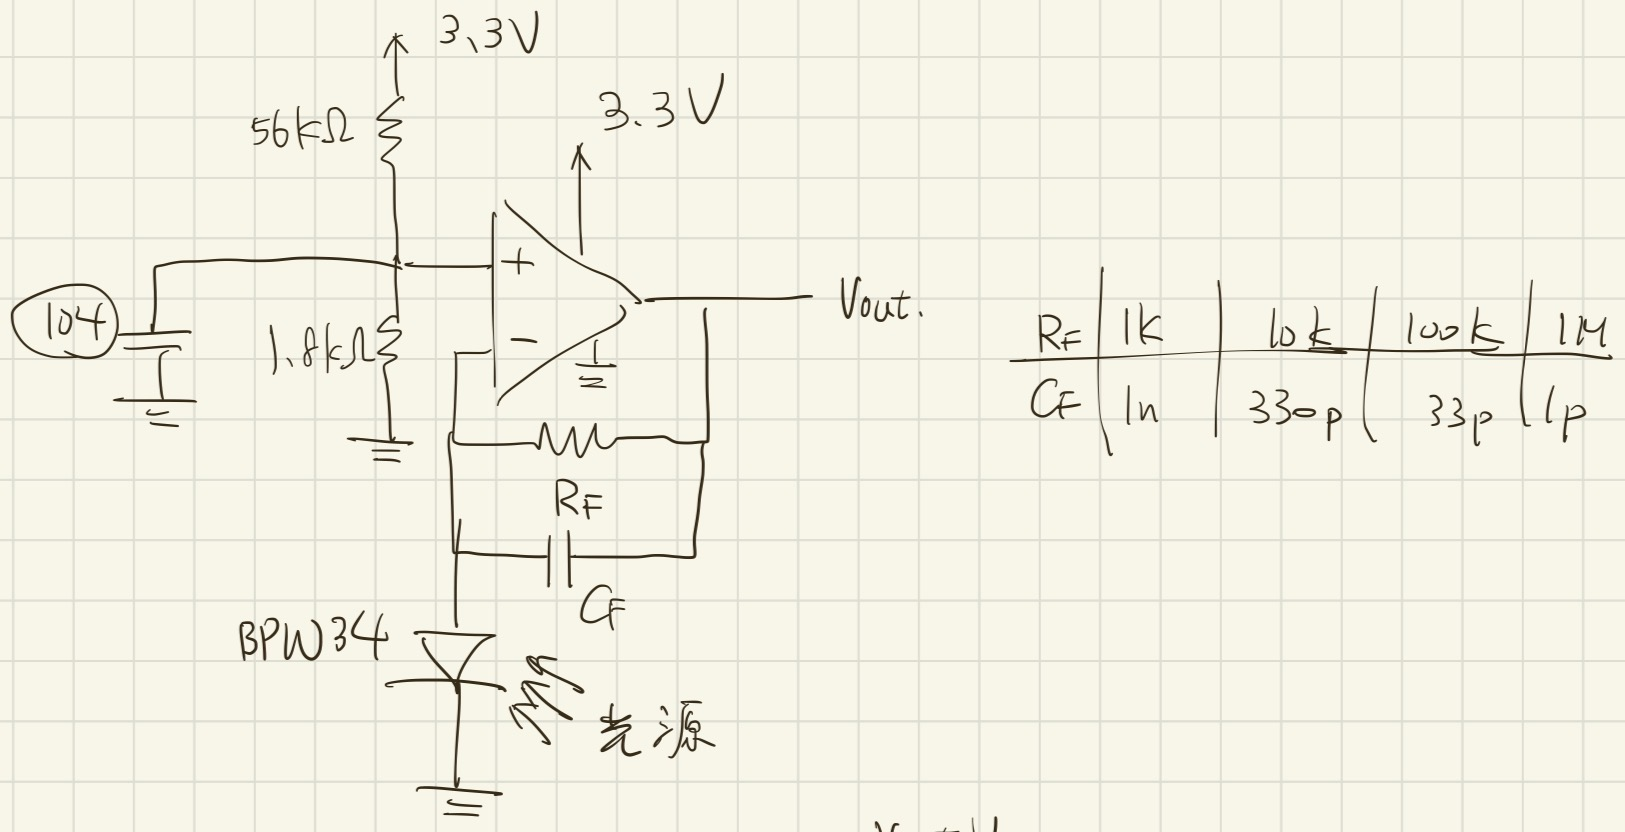
\includegraphics[width=0.9\linewidth]{2026-05-06/initial_schmatic.jpg}
  \caption{2026-05-06 麵包板 TIA 手繪圖。Op-amp 是 MCP6004,
           BPW34 接反相輸入端,非反相端透過 56 kΩ / 1.8 kΩ 分壓墊高到
           \(\sim \SI{0.103}{\volt}\)。回授 \(R_F\) 與 \(C_F\) 並聯,
           四檔增益配對見表~\ref{tab:0506-rfcf}。}
  \label{fig:0506-schematic}
\end{figure}

四檔 \(R_F / C_F\) 配對的思路是\textbf{讓 \(R_F C_F\) 乘積大致固定},
這樣每一檔的頻寬 \(f_{-3\text{dB}} = 1/(2\pi R_F C_F)\) 都落在差不多的範圍,
而不是讓低增益檔頻寬過高反而吃進更多雜訊。

\begin{table}[H]
  \centering
  \caption{四檔 \(R_F\)/\(C_F\) 配對與對應的小訊號頻寬。}
  \label{tab:0506-rfcf}
  \begin{tabular}{lllr}
    \toprule
    \(R_F\) & \(C_F\) & \(R_F C_F\) & 理論 \(f_{-3\text{dB}}\) \\
    \midrule
    1 kΩ   & 1 nF   & 1.0 μs & \(\sim\)159 kHz \\
    10 kΩ  & 330 pF & 3.3 μs & \(\sim\)48 kHz  \\
    100 kΩ & 33 pF  & 3.3 μs & \(\sim\)48 kHz  \\
    1 MΩ   & 1 pF   & 1.0 μs & \(\sim\)159 kHz \\
    \bottomrule
  \end{tabular}
\end{table}

50--150 kHz 的頻寬遠超過 20 kHz PWM 目標,所以四檔都能跑動態量測。
(註:\texttt{simulation/main.py} 的 DC 模擬為了簡化把 \(C_F\) 固定在 100 nF,
那是模擬端的近似,跟麵包板實際用的配對表不同。)

\subsection*{下午 3 點:功能驗證(手指遮光測試)}

電路接好後,先做最簡單的「手指遮光、看電表會不會動」測試,
確認光電轉換 + TIA 整條鏈路都活著。三用電表跨在 \(V_\text{OUT}\) 跟 GND 之間,
測試結果:

\begin{itemize}[leftmargin=2em,itemsep=0pt]
  \item 自然採光(無遮蔽,圖~\ref{fig:0506-light}):\(V_\text{OUT} = \SI{1.637}{\volt}\)
  \item 手指壓在 BPW34 感光面(圖~\ref{fig:0506-dark}):\(V_\text{OUT} = \SI{0.302}{\volt}\)
\end{itemize}

\(\Delta V \approx \SI{1.3}{\volt}\) 的明顯擺動,代表電路功能正確。

\begin{figure}[H]
  \centering
  \begin{minipage}{0.48\linewidth}
    \centering
    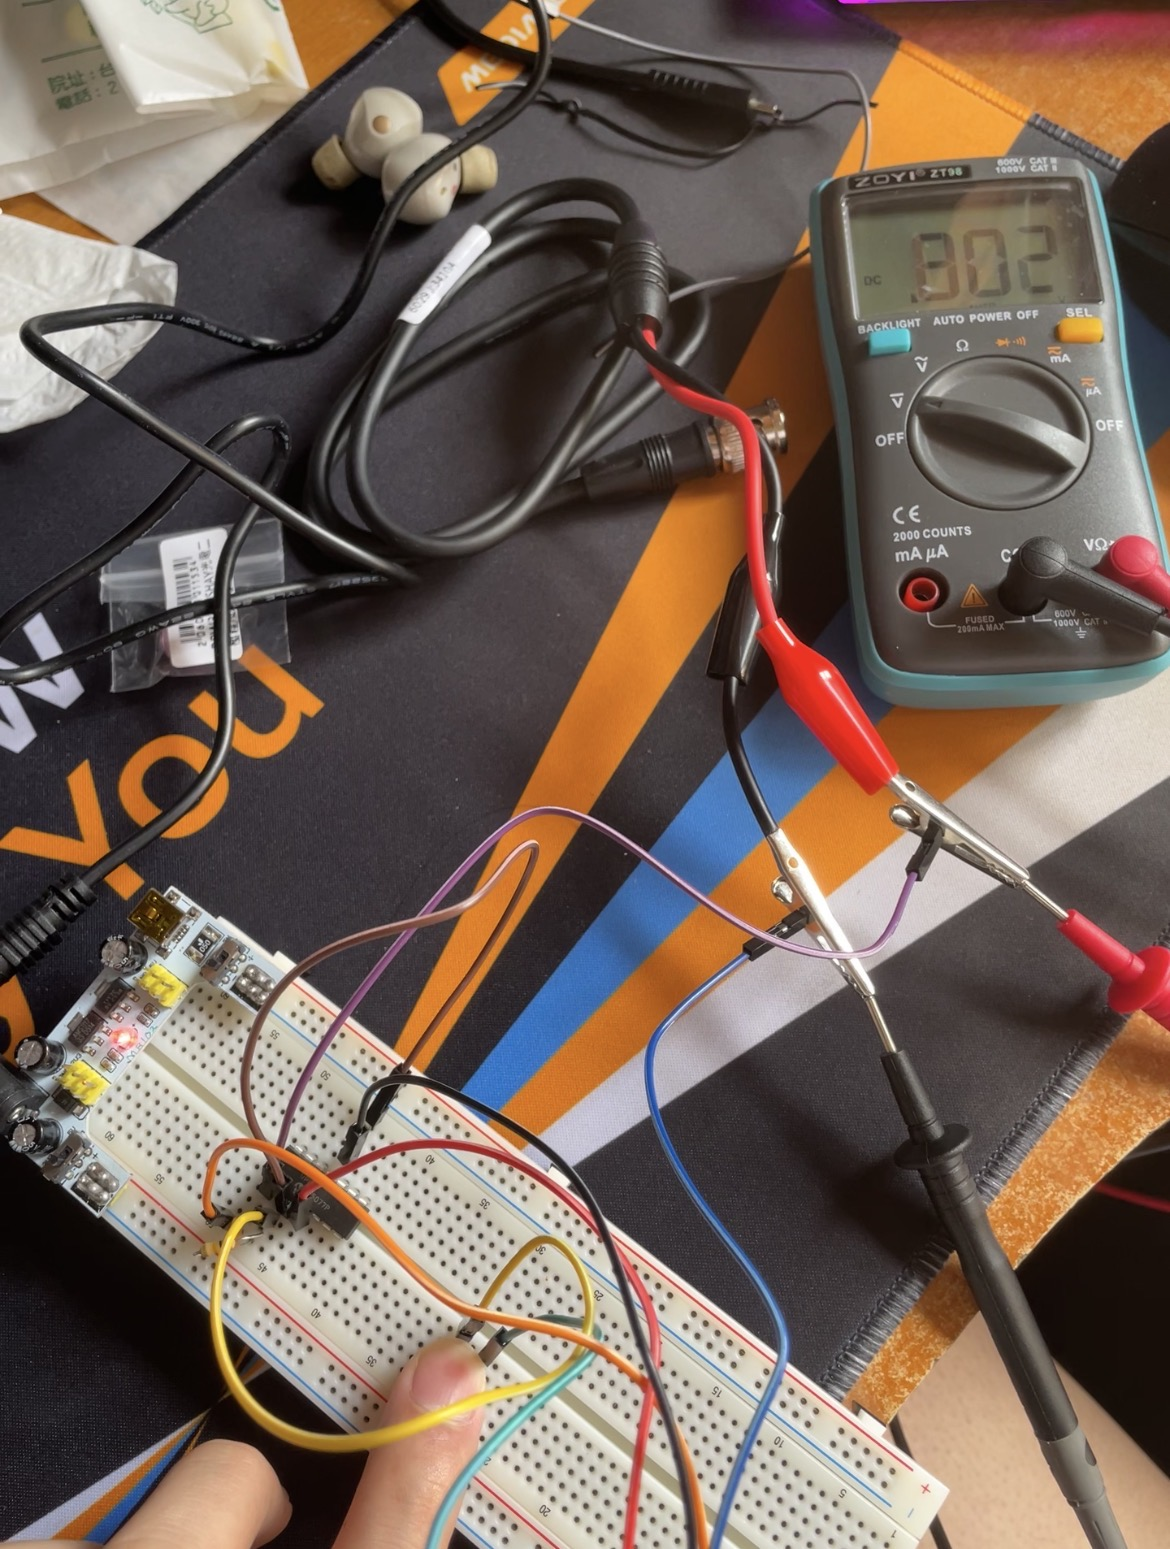
\includegraphics[width=\linewidth]{2026-05-06/BPW34_without_light.jpg}
    \caption{手指壓住 BPW34 受光面:\(V_\text{OUT} = \SI{0.302}{\volt}\)。
             無法完全壓到 \(V_\text{ref} \approx \SI{0.1}{\volt}\),
             差距來自漏光與 op-amp 的近 0 V 非線性。}
    \label{fig:0506-dark}
  \end{minipage}\hfill
  \begin{minipage}{0.48\linewidth}
    \centering
    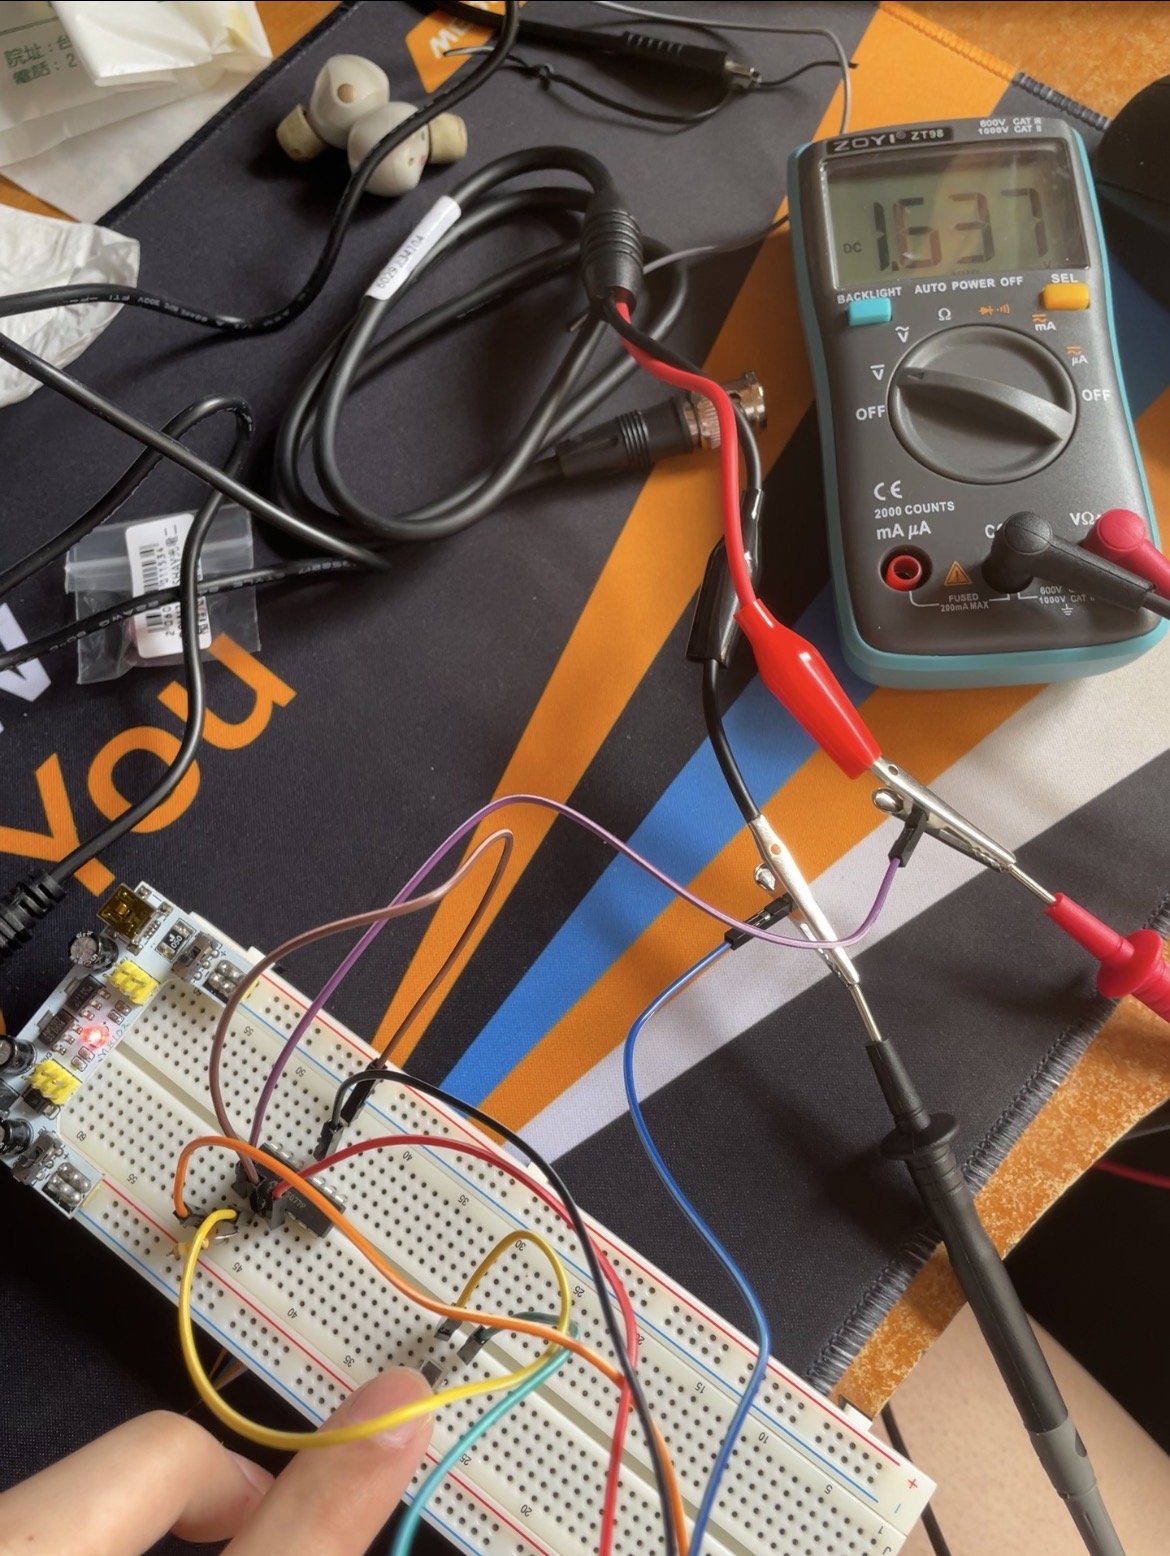
\includegraphics[width=\linewidth]{2026-05-06/BPW34_with_light.jpg}
    \caption{放開手指:\(V_\text{OUT} = \SI{1.637}{\volt}\)。
             正常室內採光下 TIA 輸出沒撞到上軌,動態範圍可用。}
    \label{fig:0506-light}
  \end{minipage}
\end{figure}

接著手動把 \(R_F\) 在四檔 \{1 kΩ, 10 kΩ, 100 kΩ, 1 MΩ\} 之間切換,
配對的 \(C_F\) 也跟著換,逐一在不同光照(全暗、白蓋、室內、手機手電筒)讀電表 ——
這就是下一節 4$\times$4 表的來源。

\subsection*{今天看到的痛點(下次採購清單)}

\begin{enumerate}[leftmargin=2em,itemsep=2pt]
  \item \textbf{杜邦線太亂}。麵包板上一旦同時掛 op-amp + 偏壓分壓 + 回授 + 量測點 + 三用電表線,
        20 cm 的杜邦線就會在板子上方繞成一坨。更糟的是,因為線太長 + BPW34 又長腳,
        \textbf{BPW34 沒辦法平貼到待測螢幕上} —— 一直被線拉住翹起來,
        感光面跟螢幕之間有明顯間隙,雜散光跑進去、訊號也不準。
        \textbf{下次採購:小跳線盒(預先剪好不同長度的硬跳線)} —— 線可以走平貼麵包板的水平路徑,
        感測元件就可以乖乖貼在螢幕上。
  \item \textbf{沒有四段波段開關}。每換一檔 \(R_F\) 都要拔線、換電阻、再插回去 ——
        4 個 \(R_F\) × 4 種光照 = 16 個讀數,每次都重接一次接線,容易插錯位、
        又會抖動電路擾動量測。
        \textbf{下次採購:1P4T 波段旋鈕開關} —— 跟 4/19 跟 Gemini 討論的方案接上,
        後續真的進外殼也用得到。
\end{enumerate}

\subsection*{量測程序與結果}

固定電路、轉動回授電阻 \(R_F\),分別在四種照度下用三用電表讀 \(V_\text{OUT}\)。原始紀錄留在
\texttt{simulation/data/exp\_260506.dat},整理表如下:

\begin{table}[H]
  \centering
  \caption{\(V_\text{OUT}\) (V) — 4 個 \(R_F\) × 4 種光照,2026-05-06 麵包板量測。}
  \label{tab:0506-bench}
  \begin{tabular}{lrrrr}
    \toprule
    \(R_F\) & Total Dark & White Cap & Room Light & Phone Flashlight \\
    \midrule
    1 MΩ    & 0.318  & 3.33   & 3.33   & 3.33  \\
    100 kΩ  & 0.024  & 0.523  & 1.342  & 3.33  \\
    10 kΩ   & 0.0031 & 0.0485 & 0.1352 & 2.40  \\
    1 kΩ    & 0.0058 & 0.0047 & 0.0113 & 0.214 \\
    \bottomrule
  \end{tabular}
\end{table}

每一個讀數 \(\SI{3.33}{\volt}\) 都是頂到電源軌的 clipping。

\subsection*{模擬 vs 量測比對}

PySpice 端跑 \texttt{simulation/main.py},四條 \(R_F\) 的 DC sweep \(V_\text{OUT}(I_\text{photo})\)
如圖~\ref{fig:0506-tia-sweep}。

\begin{figure}[H]
  \centering
  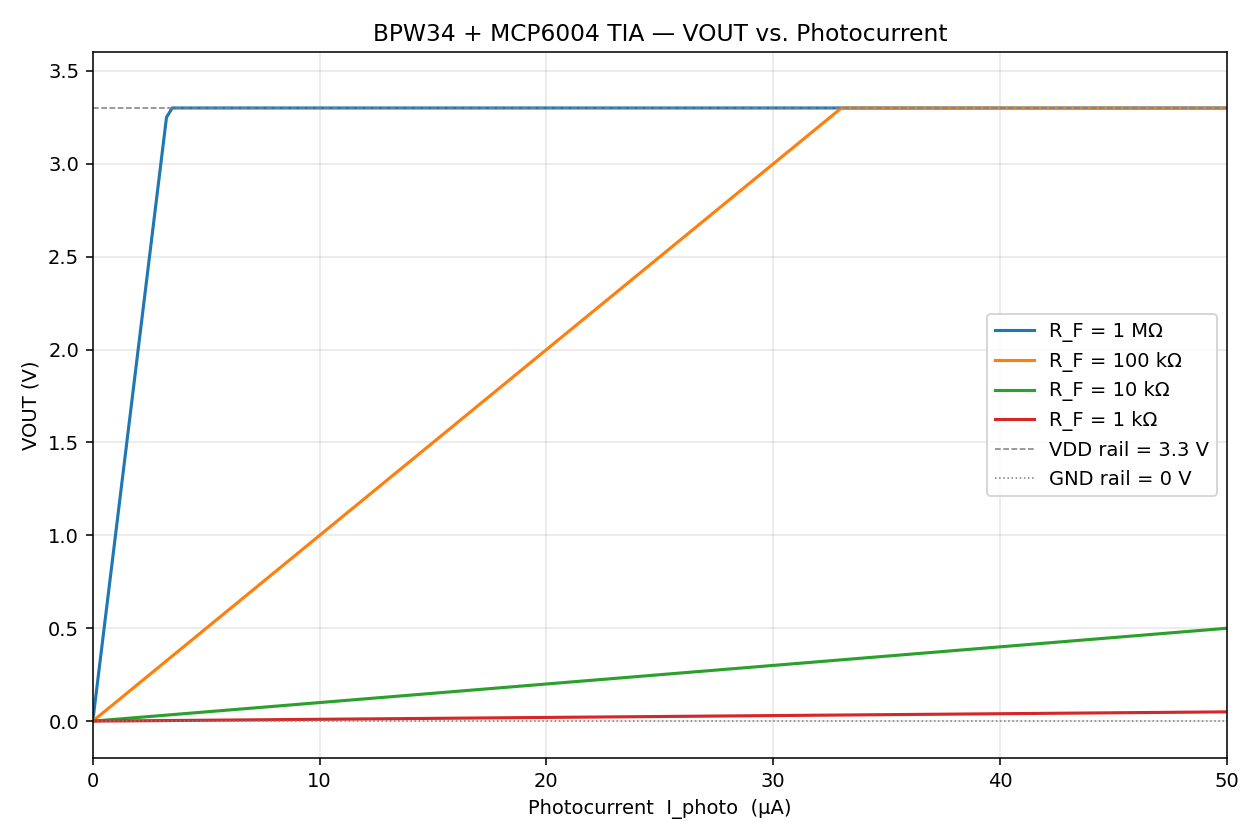
\includegraphics[width=0.85\linewidth]{2026-05-06/tia_sweep.png}
  \caption{PySpice DC sweep:四個 \(R_F\) 對應的 \(V_\text{OUT}\) vs \(I_\text{photo}\),
           上下軌位 0 V 與 \(V_{DD} = \SI{3.3}{\volt}\) 標出。 模擬完美呈現
           \(V_\text{OUT} = I_\text{photo} R_F\) 直到撞到上軌為止。}
  \label{fig:0506-tia-sweep}
\end{figure}

兩個對照點讓我們確認模擬與實際對得上:

\begin{itemize}[leftmargin=2em,itemsep=0pt]
  \item \textbf{線性增益}(Room Light 那一欄,100 kΩ 與 10 kΩ 都沒飽和):
        \(V_\text{OUT}\) 比值 \(1.342 / 0.1352 = 9.93\),對「理想 10×」誤差不到 1\%。
        反推光電流 \(I_\text{photo} = 13.42\) μA 與 \(13.52\) μA — 兩個獨立 \(R_F\)
        對同一物理量的估計差 0.7\%。
  \item \textbf{Clipping ceiling}:所有飽和讀值都落在 3.33 V,與模擬的 3.3 V 軌位
        差 30 mV(在三用電表標稱準度內)。每個 \(R_F\) 的 \(I_\text{clip} = V_{DD}/R_F\)
        都和飽和欄位一一對應 — \(R_F = 1\) MΩ 對應 \(I_\text{clip} = \SI{3.3}{\micro\ampere}\),
        一點點室內光就過頭;\(R_F = 1\) kΩ 對應 \(\SI{3.3}{\milli\ampere}\),手機手電筒
        近距離照都還在線性區。
\end{itemize}

\subsection*{非理想項解釋:為什麼 Total Dark 不是 0 V}

模擬下 \(I_\text{photo} = 0\) 給 \(V_\text{OUT} = 0\),但 bench 不是。把全黑欄位除以
\(R_F\) 反推 apparent input current:

\begin{itemize}[leftmargin=2em,itemsep=0pt]
  \item 三個高阻檔(1 MΩ / 100 kΩ / 10 kΩ)反推都是 \(\approx 250\)--\(320\) nA。
        \textbf{固定電流被 \(R_F\) 線性放大}的特徵,不是固定電壓 offset。
        最合理的來源是 \textbf{stray ambient light leakage} —— 房間光、電表 LED、
        手機螢幕的微弱漏光,任何一個都足以在 BPW34 的 \(\SI{7.5}{\square\milli\metre}\)
        感光窗上產生幾百 nA 的光電流(對應 μW 量級的光功率)。
  \item \(R_F = 1\) kΩ 時 \(V_\text{OUT}\) 升到 \(\SI{5.8}{\milli\volt}\) — 比理論 dark 還大,
        這時主導的是 \textbf{MCP6004 的輸入失調電壓 \(V_{os}\)}(spec 標 ±2 mV typical、
        ±4.5 mV max),不是光電流。在低 \(R_F\) 把光電流項壓下去後,
        op-amp 自身的 offset floor 才浮現。
\end{itemize}

把這兩個非理想項加進 PySpice 的網表很容易,但今天先停在「指認來源」這一步。

\subsection*{動態特性:用模擬挑 \(C_F\)}

固定 \(R_F = 100\) kΩ,把 \(C_F\) 掃 \{1 pF, 10 pF, 100 pF, 1 nF, 100 nF\},
跑 AC sweep(1 Hz–1 MHz)看 \(|Z(f)|\)、再跑 20 kHz 0–10 μA 方波 transient 看波形:

\begin{figure}[H]
  \centering
  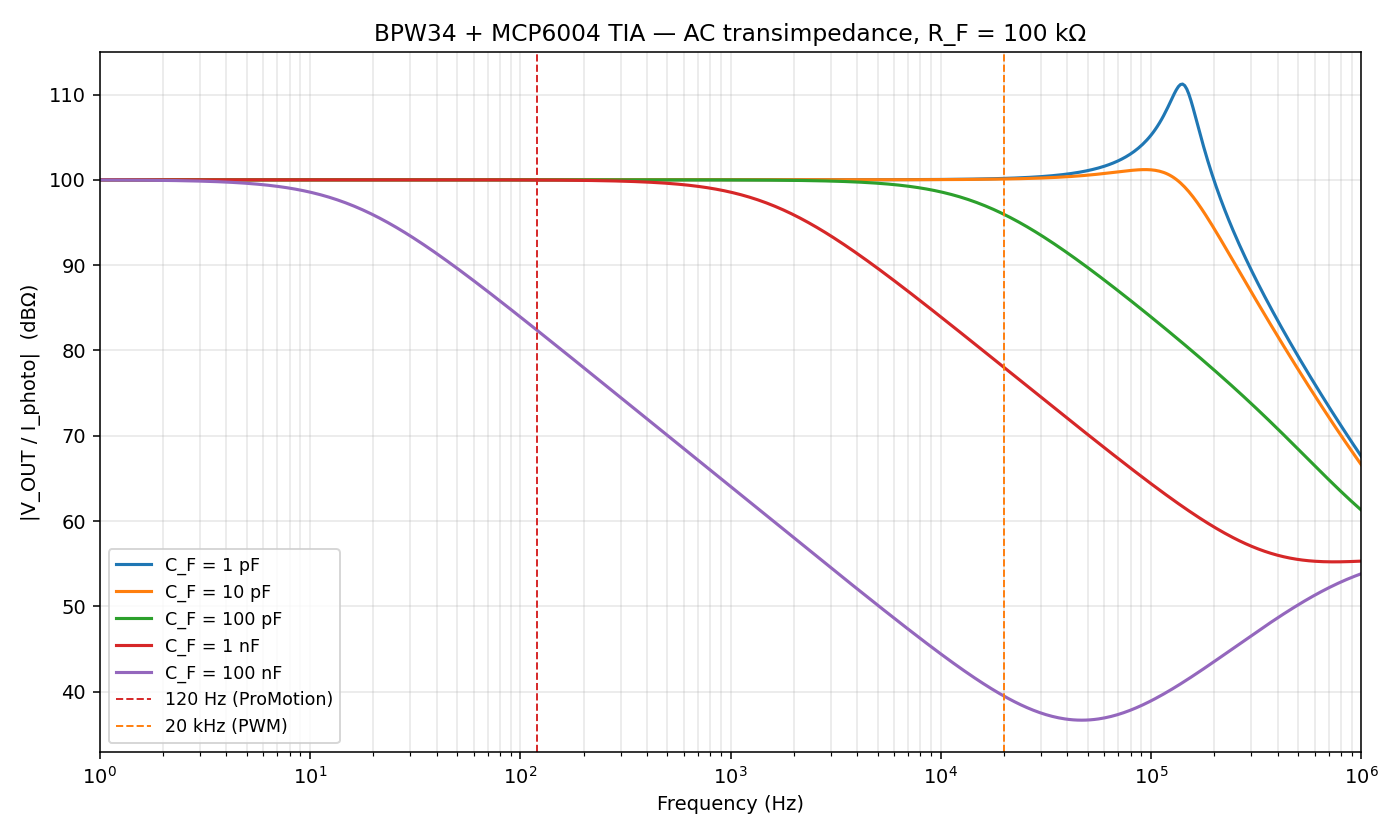
\includegraphics[width=0.85\linewidth]{2026-05-06/ac_bode.png}
  \caption{AC transimpedance \(|V_\text{OUT}/I_\text{photo}|\)。標出 120 Hz(ProMotion)
           與 20 kHz(PWM)兩個目標頻率。}
  \label{fig:0506-bode}
\end{figure}

\begin{figure}[H]
  \centering
  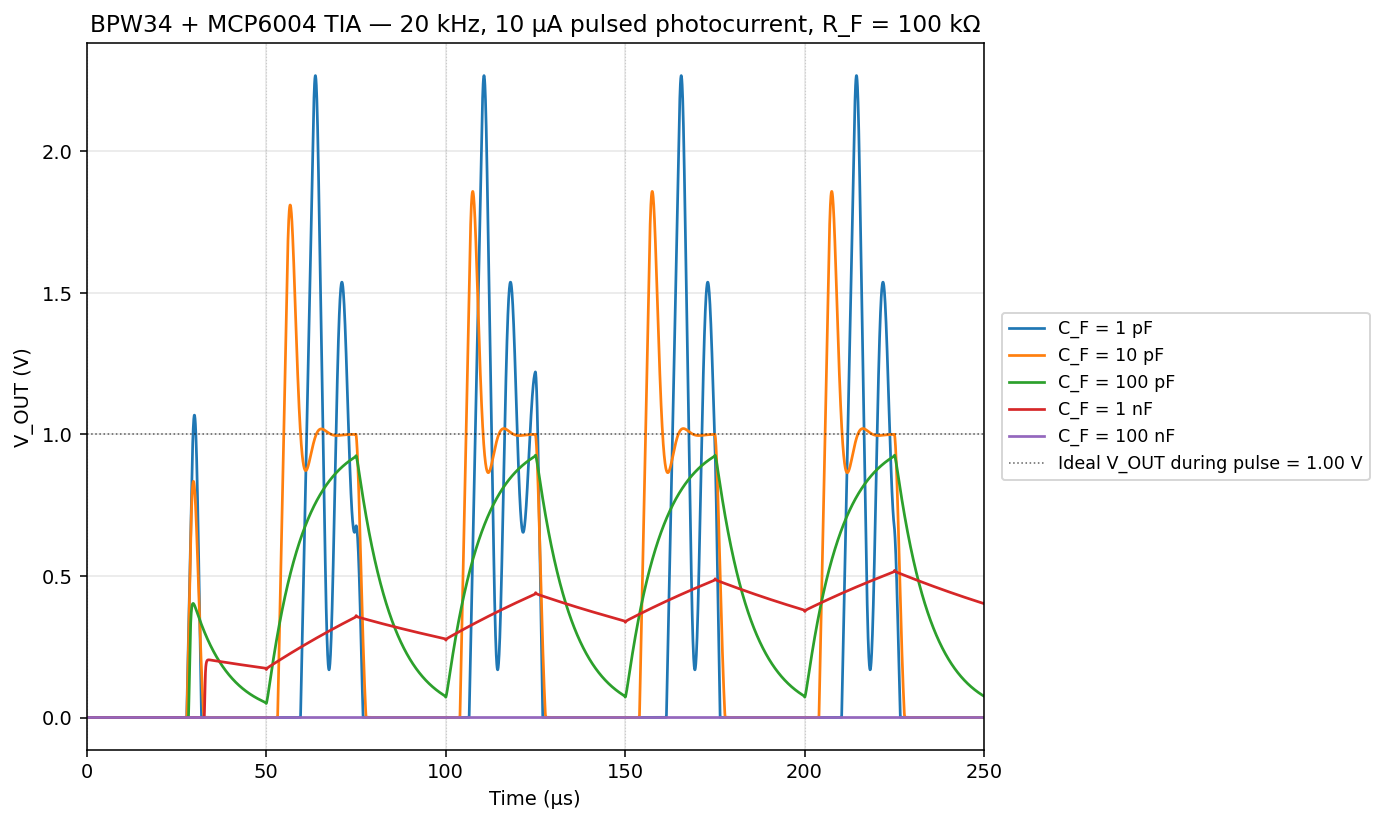
\includegraphics[width=0.85\linewidth]{2026-05-06/transient_pwm.png}
  \caption{20 kHz、10 μA 方波光電流的 transient 響應。理想 \(V_\text{OUT} = 1.0\) V。
           \(C_F = 1\) pF 嚴重 ringing、\(C_F \geq \SI{1}{\nano\farad}\) 變積分波形,
           中間的 10 pF 邊緣銳利又穩定。}
  \label{fig:0506-transient}
\end{figure}

從 Bode 跟 transient 一起看,各個 \(C_F\) 對兩個目標頻率的可用性:

\begin{table}[H]
  \centering
  \caption{\(R_F = 100\) kΩ 下,各補償電容 \(C_F\) 的可用性。}
  \label{tab:0506-cf}
  \begin{tabular}{lrcc}
    \toprule
    \(C_F\) & 模擬 \(f_{-3\text{dB}}\) & 120 Hz(ProMotion) & 20 kHz(PWM) \\
    \midrule
    1 pF   & 224 kHz           & 通過 & 通過(欠補償、有 ringing) \\
    \textbf{10 pF}  & \textbf{170 kHz} & \textbf{通過} & \textbf{通過(推薦)} \\
    100 pF & 16 kHz            & 通過 & 衰減 \(\sim\)\(-3\) dB,可用 \\
    1 nF   & 1.6 kHz           & 通過 & 砍掉 \\
    100 nF & 16 Hz             & 砍掉 & 砍掉 \\
    \bottomrule
  \end{tabular}
\end{table}

\textbf{推薦 \(C_F = 10\) pF}:既能保住 20 kHz PWM 邊緣,又比 1 pF 更穩、不會 ringing。
而今天 bench 上用的 \(C_F = \SI{100}{\nano\farad}\) 把 \(f_{-3\text{dB}}\) 壓到 16 Hz,
把 120 Hz 跟 20 kHz 兩個目標都吃掉了 —— 純 DC 量測沒事,但下次做動態量測前必須換掉。

\subsection*{今日心得}

\begin{itemize}[leftmargin=2em,itemsep=0pt]
  \item \textbf{TIA 理論驗證成功}:兩個獨立 \(R_F\) 對同一光電流的估計差 0.7\%、
        \(V_\text{OUT}\) 比值與 \(R_F\) 比值對到 1\% 內、clipping ceiling 與 \(V_{DD}\)
        對到 1\% 內 —— PySpice 跟麵包板真的對得起來,這份信心很關鍵。
  \item \textbf{Dark floor 不是 bug}:300 nA stray ambient + 5.8 mV \(V_{os}\) 都是
        datasheet 可查的真實效應,不是電路接錯。日後要進低光量測,得加遮光罩
        並且軟體做開機暗態校正。
  \item \textbf{\(C_F\) 是我 4/19 沒考慮到的東西}:4/19 只決定 \(R_F\) 用旋鈕切檔,
        以為 \(C_F\) 隨便挑。今天才知道 \(C_F = \SI{100}{\nano\farad}\)
        會把動態目標砍光,要改成 \(\sim \SI{10}{\pico\farad}\)。
  \item \textbf{ngspice + macromodel + PySpice 三層膠水}:libngspice SONAME、
        \texttt{set ngbehavior=ps} 時機、\texttt{Note:} 被當 fatal 這三個坑要記住,
        日後換機器重建環境一定會再撞。
  \item \textbf{下一步}:做動態量測前要先換 \(C_F\) 為 10 pF;同時開始想 Pico ADC
        的取樣率與 buffer 大小(2 kHz 對 ProMotion 1 Hz 需要長窗,10 kHz 對 PWM
        20 kHz 需要短窗,要兩套參數還是動態切換,還沒想清楚)。
\end{itemize}
